\documentclass{X:/Documents/Coding/Latex/myassignment}
\title{Brief Analysis of Norovirus Data}
\usepackage{biblatex}
\addbibresource{sources.bib}

\begin{document}

\maketitle
\setlength{\parindent}{0pt}
An in depth study on norovirus outbreaks in hospital settings, with one of three intervention strategies put in place (including control). Using resources from Gaythorpe\parencite{dynamics}\parencite{model}, the SA health department\parencite{SAHD} and Ross et al\parencite{BLACK2015159}, a statistical model is derived to calculate the infectivity of the disease within hospitals. The study finds that each individual who is infected is expected to infect another $2$ people. Or specifically, the reproduction number (the expected number of people infected by one individual) is approximately $2.2883$ when there is no intervention strategy ($T_0$). When the strategy $T_1$ is put in place, This value is reduced to approximately $1.9242$, corresponding to the expectation that an individual will infect just under two people over their infectious period. This is an improvement on $T_0$, and hence intervention will help reduce the effect of norovirus outbreaks. Intervention strategy two, $T_2$, reduces the value to approximately $1.5518$. This is a much greater improvement on the control, and hence strategy $T_2$ should be put in place. 

These values are obtained using a statistical estimate, and obtaining the average (modal) value. The distributions for $R_0$, $\alpha_1$ and $\alpha_2$ are shown in figure~\ref{fig:density}, where $R_0$ is the reproduction number, $\alpha_1$ and $\alpha_2$ multiply with $R_0$ to get the effective reproduction numbers under $T_1$ and $T_2$ respectively. 
The values stated above correspond to the peaks on these plots, but it is worth acknowledging that there is a reasonable probability that $R_0$ could be between $2$ and $2.6$ and $\alpha_1$ could even be greater than $1$, corresponding to an \textit{increase} in infectivity under $T_1$.

\vspace{2em}

As a result of this analysis, more alternative intervention strategies should be investigated. In the meantime, intervention strategy $T_2$ should be put in place as it will greatly decrease the spread of norovirus within hospital environments. 


\begin{figure}[tb]
	\centering
	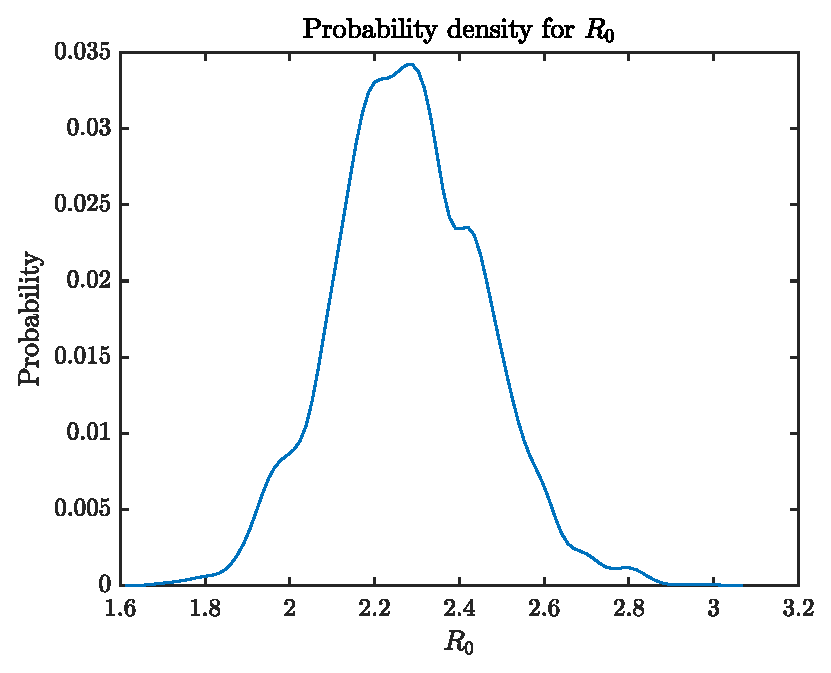
\includegraphics[width=0.45\linewidth]{Probdensity1.eps}
	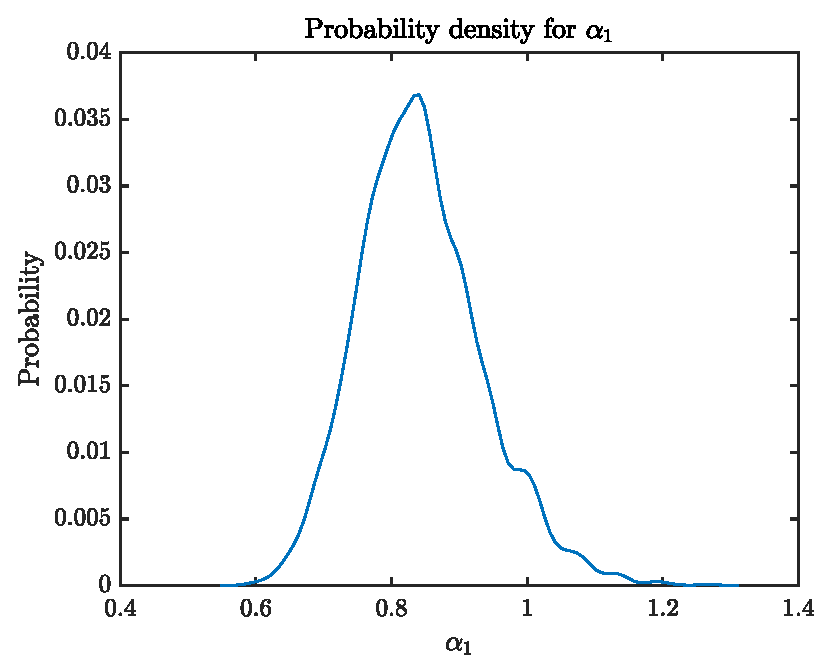
\includegraphics[width=0.45\linewidth]{Probdensity2.eps}
	\includegraphics[width=0.45\linewidth]{Probdensity3.eps}
	\caption{Probability density curves for the parameters - the horizontal axis is the parameter while the vertical is the probability}
	\label{fig:density}
\end{figure}



\appendix

\printbibliography

\end{document}